\documentclass[12pt]{article}
\title{Project 3}
\author{Eirik Ramsli Hauge\\
Joakim Kalsnes
}
\date{\today}

\usepackage{amsmath}
\DeclareMathOperator*{\argmin}{argmin}
\usepackage{bm}
\usepackage{xcolor}
\usepackage{hyperref}
\usepackage[english]{babel} 
%\usepackage{fullpage} 
\usepackage{amsfonts} 
\usepackage{amssymb} 
\usepackage{verbatim} 
 
\usepackage{color} 
\usepackage{setspace} 
\usepackage{blindtext}
\usepackage{epstopdf} 
\usepackage{braket}

\usepackage{cite} 
\usepackage{caption}
\usepackage{subcaption}
\usepackage{upgreek}
\usepackage{array,multirow}
\usepackage{pdfpages}

\usepackage{graphicx} 
\usepackage{float}

\usepackage{nameref}
\usepackage{hhline}
\usepackage{xtab}
\usepackage{booktabs, makecell, longtable}
\usepackage{lscape}

\numberwithin{figure}{section}

\newcommand{\husk}[1]{\color{red} #1 \color{black}}
\newcommand{\sjekk}[1]{\color{violet} #1 \color{black}}

\begin{document}
\maketitle

\section{Theory}
For this project we are going to use logistic regression, neural networks and random forest to analyse the credit card example. Logistic regression and neural networks were described in project 2 (\husk{reference}). This theory section will therefore focus on random forest, starting with a presentation of decision trees.
\subsection{Decision Trees}
This section will follow closely the description of decision trees in chapter 6 of Géron's book [\husk{reference}].\\
Decision trees is a type of Machine Learning algorithm that can be used for both regression and classification. They are easy to interpret and intuitive in the way the algorithm is constructed. As we will see in the next section, they are the fundamental components of random forests. To understand how decision trees work, we start by looking at an example. Figure \ref{figT:iris_tree} shows a decision tree made on the classic iris dataset using Scikit-Learn (taken from Géron p. 170 [\husk{reference}]). The goal of the model is to classify an iris flower. When we have a new flower, we start at the \textit{root node} (depth=0) and ask if the petal length is smaller than 2.45 cm. If it is, we move down the tree to the left child node (depth=1, left). In this example, it is a leaf node, that is it does not have any children nodes. From this lead node we see that the decision tree predicts that the flower is and Iris-setosa (class=setosa). If the petal length is longer than 2.45 cm we move to the root's right child node (depth=1, right). This is not a leaf node, so it asks a new question: is the flower's petal width smaller than 1.75 cm? If it is, then the flower is most likely of class Versicolor. If it is not, it is most likely of class Virginica.\\ 
\begin{figure}[H]
\centering
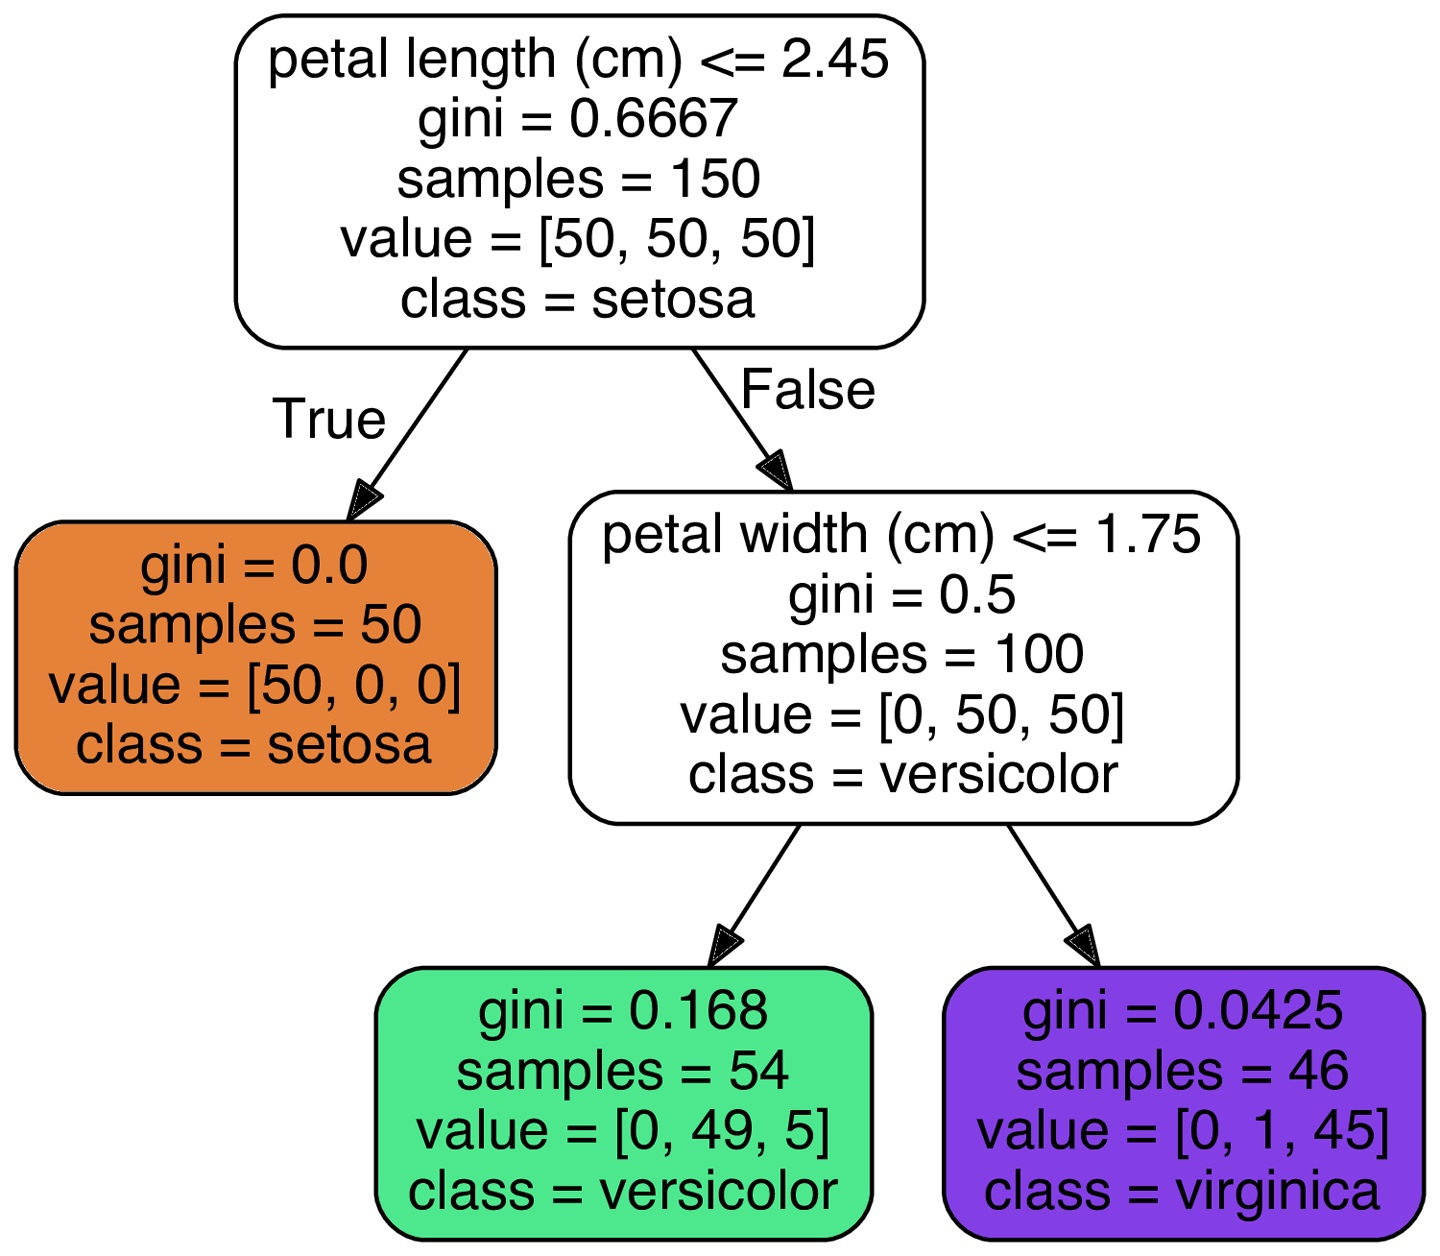
\includegraphics[width=0.8\linewidth]{decision-tree-iris.jpg}
\caption{Iris Decision Tree}
\label{figT:iris_tree}
\end{figure}
\noindent
A node's \textit{samples} attribute counts how many training instances it applies to. For example, in Figure \ref{figT:iris_tree}, 50 training instances have a petal length smaller than 2.45 cm. The \textit{value} attribute tells us how many training instance of each class this node applies to. For example, the bottom left applies to 0 Iris-Setosa, 49 Iris-Versicolor and 5 Iris-Virginica. The \textit{class} gives the most likely class, i.e. the class with the highest count in \textit{value}. We can also get the probability of each class as an output (not shown in Figure \ref{figT:iris_tree}). The probability is simple the ratio of class instances among the training instances in the given node. For example in (depth 2, left), the probabilities are: p(class=setosa) = 0/54, p(class=versicolor) = 49/54 and p(class=virginica) = 5/54. Finally, a node's \textit{gini} attribute measures its \textit{impurity}. A node is "pure" ($gini=0$) if all training instances it applies to belong to the same class, e.g. (depth 1,left) in figure \ref{figT:iris_tree}. The gini score, G$_i$, is calculated using the following equation:
\begin{equation}
G_i = 1 - \sum_{k=1}^{n}{p_{i,k}}^2,
\label{eqT:gini_score}
\end{equation}
where $p_{i,k}$ is the ratio of class $k$ instances among the training instances in the $i^{th}$ node. As an example, the gini score of (depth 2, right) is: $1-(0/46)^2-(1/46)^2-(45/46)^1 \approx 0.0425$. \\ \\
To train, or "grow", decision trees, Scikit-Learn uses the \textit{Classification and Regression Tree} (CART) algorithm. The algorithm first splits the training set in two subsets using a single feature $k$ and a threshold$t_k$. To choose $k$ and $t_k$, the algorithm searches for the pair $(k, t_k)$ that produces the purest subsets. The cost function to minimize is given by the following equation:
\begin{equation}
J(k,t_k) = \frac{m_{left}}{m}G_{left}\ +\ \frac{m_{right}}{m}G_{right},
\label{eqT:CART_cost}
\end{equation}
where $G_{left/right}$ measures the impurity of the left/right subset and $m_{left/right}$ is the number of instances in the left/right subset. The Gini impurity measure (equation \ref{eqT:gini_score}) is used by default, but one can also use entropy impurity defined by:
\begin{equation}
H_i = - \underbrace{\sum_{k=1}^{n} p_{i,k}log(p_i{i,k})}_{p_{i,k}\neq0},
\label{eqT:entropy_cost}
\end{equation}
where $p_{i,k}$ is the same as in equation \ref{eqT:gini_score}. Once the algorithm has split the training set in two subsets, it splits the subsets using the same logic, then the sub-subsets and so on. The algorithm will stop when it cannot find a split that reduces the impurity or when it reaches the maximum depth, which is a hyperparameter set by the user. \\ \\
Decision trees make very few assumptions about the training data. If no constrain is set on the algorithm, it will likely adapt the tree structure very well to the training data. This will however most likely lead to overfitting, and the tree will generalize poorly to test data. To avoid overfitting, we therefore need to restrict, regularize, the decision tree. One way is by restricting the maximum depth of the tree, where a lower maximum depth reduces the risk of overfitting. Other parameters that restrict the shape of the decision tree is:\\
$\bullet$ Minimum number of samples a node must have before it can be split.\\
$\bullet$ Minimum number of samples a leaf node must have (absolute number or fraction of total instances).\\
$\bullet$ Maximum number of leaf nodes.\\
$\bullet$ Maximum number of feature that are evaluated for splitting at each node.\\ \\
We will only use decision tress and random forests for classification, but we mention briefly here that can be used for regression as well. The algorithm, and hence the decision trees, are very similar to the classification case. The regression prediction will simply be the average value of the training instances in the leaf node you end up in. The splitting is now done in way that minimizes the mean squared error (MSE) rather than the impurity.\\ \\
The main issue with decision trees is that are very sensitive to small variations in the training data. Just removing or adding one sample, may change the tree completely. In addition, since the Scikit-Learn model is stochastic we might get very different models on the same training set.  Random forests limits this instability by averaging over many trees.\\ \\

\subsection{Random Forests}
This section is heavily based on chapter 7 about ensemble learning and random forests in Géron's book [\husk{reference}].\\
The idea behind random forests is simple: You train a group of decision trees, each on a different random subset of the training set. To make predictions, you obtain the predictions from all individual trees, then predict the class that gets the most votes. Random forests is an \textit{Ensemble method}, where an \textit{ensemble} in machine learning is  a group of predictors.\\ \\
When making the prediction, there are different ways of counting the votes. One can use either \textit{hard voting} or \textit{soft voting}. Hard voting is the most straightforward method where you just count the number of predictors that predict each class, and choose the class that got the most votes. In soft voting, we use the probability of each class. The class probabilities are found from averaging the predicted probability over all individual predictors. To predict the class, we then use the class with the highest class probability. Soft voting gives more weight to highly confident votes, and therefore often achieves higher performance than hard voting.\\ \\


\section{Discussion}
Interpretability of models. White box vesus black box (Géron p. 172).

\end{document}